\documentclass[12pt,portrait]{article}
\usepackage{cite}
\usepackage{wrapfig} 
\usepackage{url}
\usepackage{graphicx}
\usepackage{amsmath}
\usepackage{amsfonts}
\usepackage{amssymb}
\usepackage{geometry}
\geometry{verbose,letterpaper}
\usepackage{media9}
\usepackage[english]{babel}
\usepackage{hyperref}
\usepackage{placeins}
\usepackage{subcaption}
\usepackage{multirow}
\usepackage{rotating}

\title{Linear Algebra for Computational Engineering}
\date{}
\author{Stephen Wood}


\begin{document}
\maketitle

%A library of linear algebra software for the solution of computational engineering problems is not a 
%novel or unique resource.
A library that provides accurate answers, effectively utilizes modern architectures, enable solver 
development, facilitates software maintenance, and reduces the time to solution for finite element 
discretizations is not easy to find.
The outline of a linear algebra library designed for integration in the workflows of finite element software is presented.
The convergence of the Flexible GMRES Method variants implemented in LACE and the FGMRES implementation within Intel's 2017 Math Kernel Library for a benchmark problem from the field of computational fluid dynamics are also presented. 

\section{Motivation}
To wholly harness current and emerging high performance computer architectures CFD software 
needs to utilize multilevel decomposition across nodes with fine grained parallelism on threads of a 
CPU or accelerator. 
In particular the residual calculation needs graph coloring per subdomain for effective multi-threading.  
Subtle variations in work sharing patterns have consequences for numerics, algorithmic performance, 
and time to solution. 
A resource of linear algebra components tailored for modern architectures and extensible to emerging 
architectures will be useful for the development and modernization of finite element software. 
Such a library will be a contribution to the field of computational fluid dynamics.  
This is the goal of the Linear Algebra for Computational Engineering (LACE) Library.

\FloatBarrier
\section{LACE Library Overview}

An outline of the LACE library is shown in Figure \ref{fig:LACE}.
Many of the elements shown in Figure \ref{fig:LACE} have been implemented.
Those elements that are planned for future releases are denoted with (future) on the outline.

As an example of a specific implementation, a more detailed view of the Generalized Minimal Residual Method within LACE is shown in Figure \ref{fig:LACE_GMRES}.

%\begin{figure}[ht]\centering
%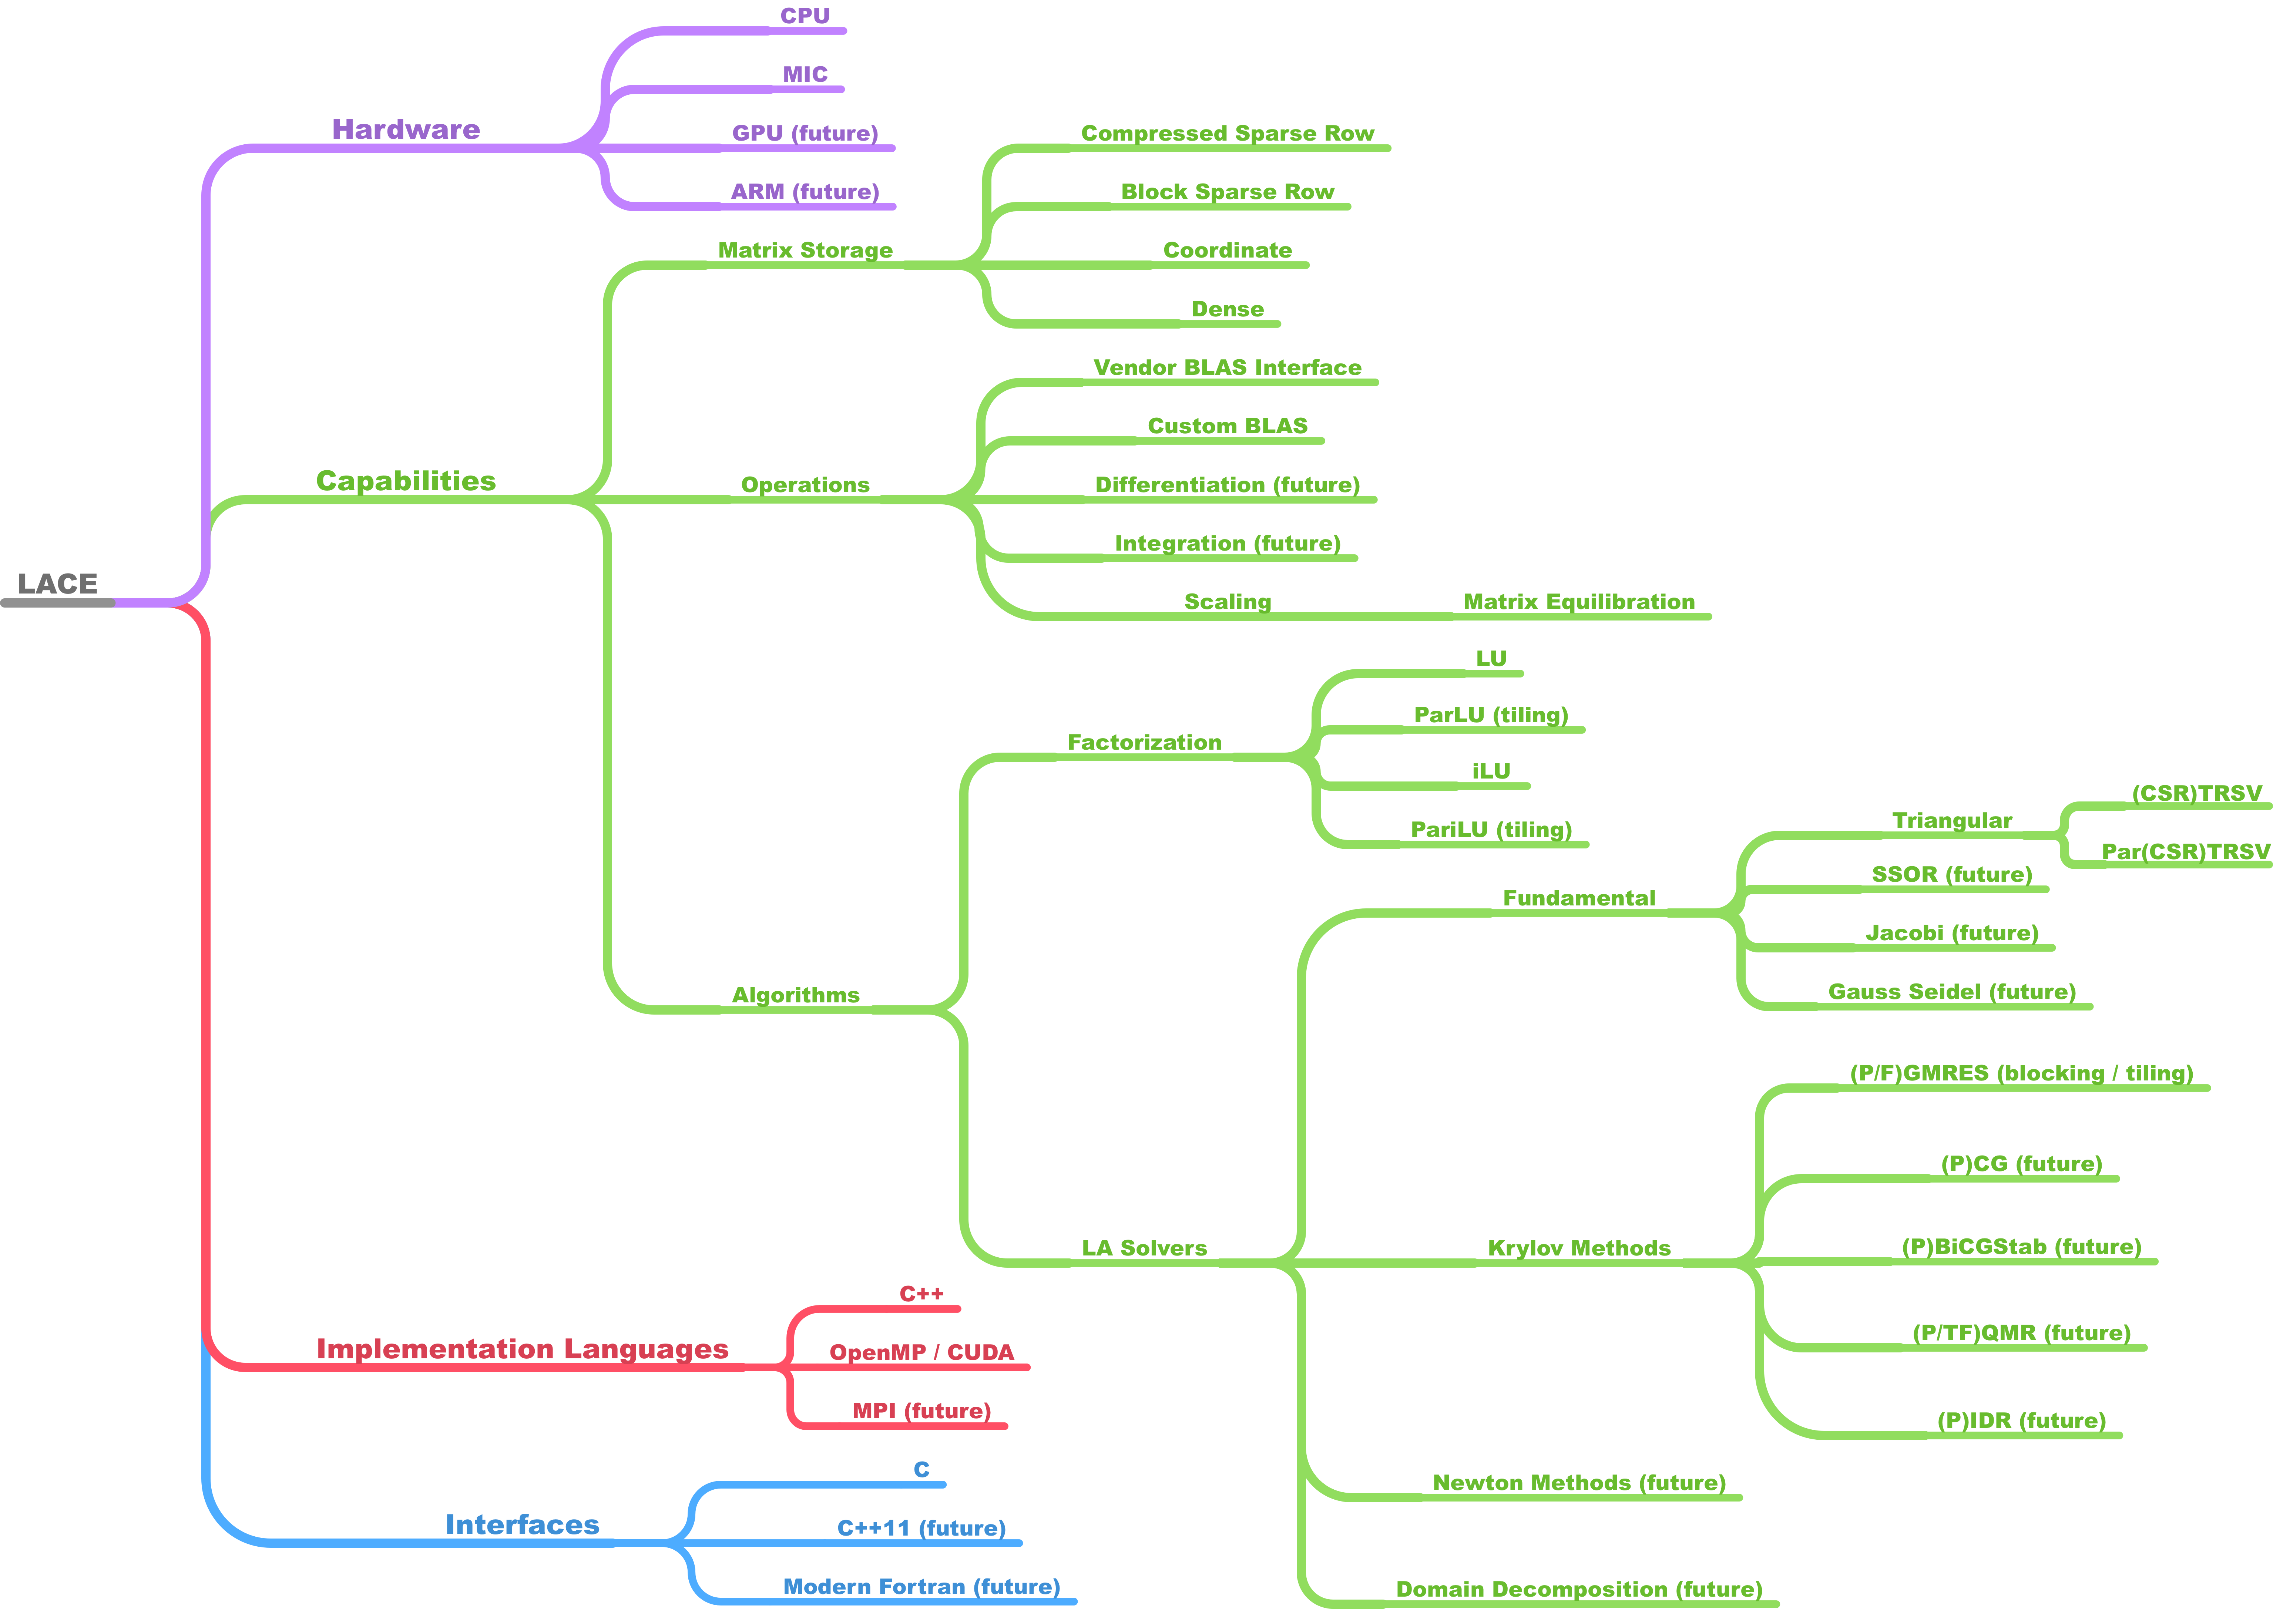
\includegraphics[width=0.95\columnwidth]{../images/LACE_1b.png}
%\caption{Outline of significant features of LACE that have been realized or are planned for future release.}
%\vspace{-10pt}
%\label{fig:LACE}
%\end{figure}

\begin{sidewaysfigure}[ht]\centering
  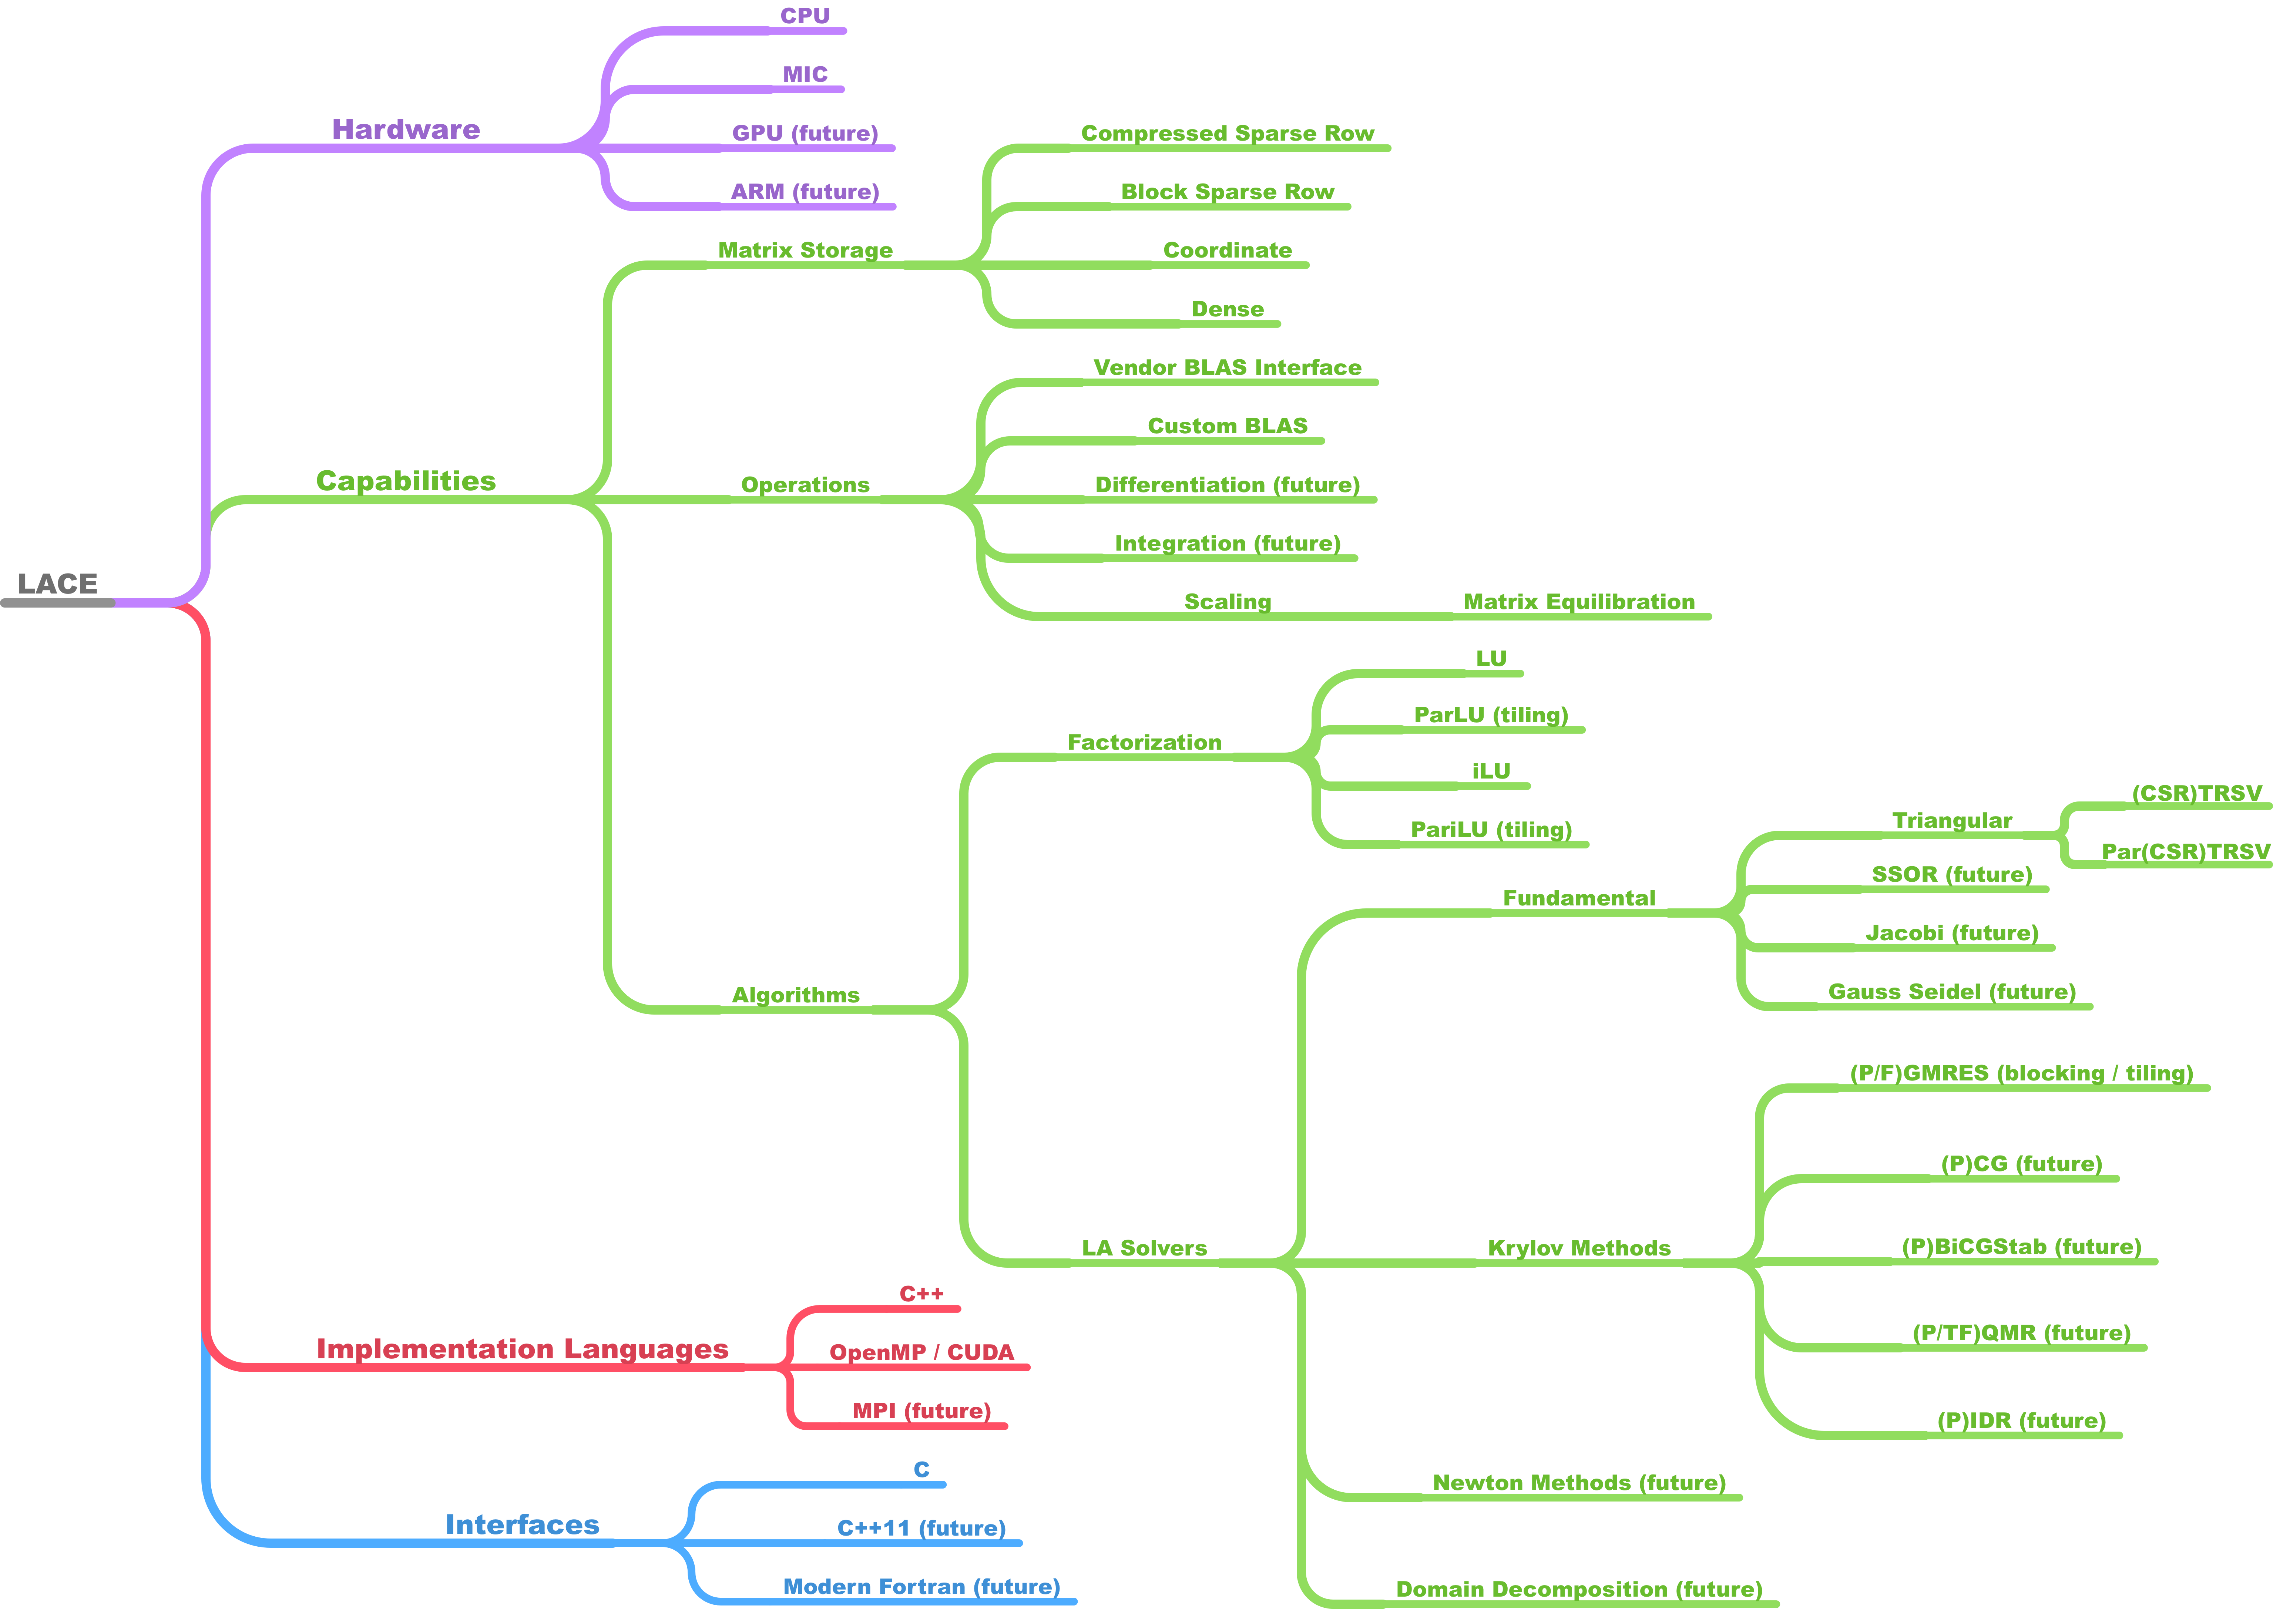
\includegraphics[width=\columnwidth]{../images/LACE_1b.png}
  \caption{Outline of significant features of LACE that have been realized or are planned for future release.}
  \vspace{-10pt}
  \label{fig:LACE}
\end{sidewaysfigure}

%\FloatBarrier
%\section{(P/F)GMRES}

\begin{sidewaysfigure}[ht]\centering
  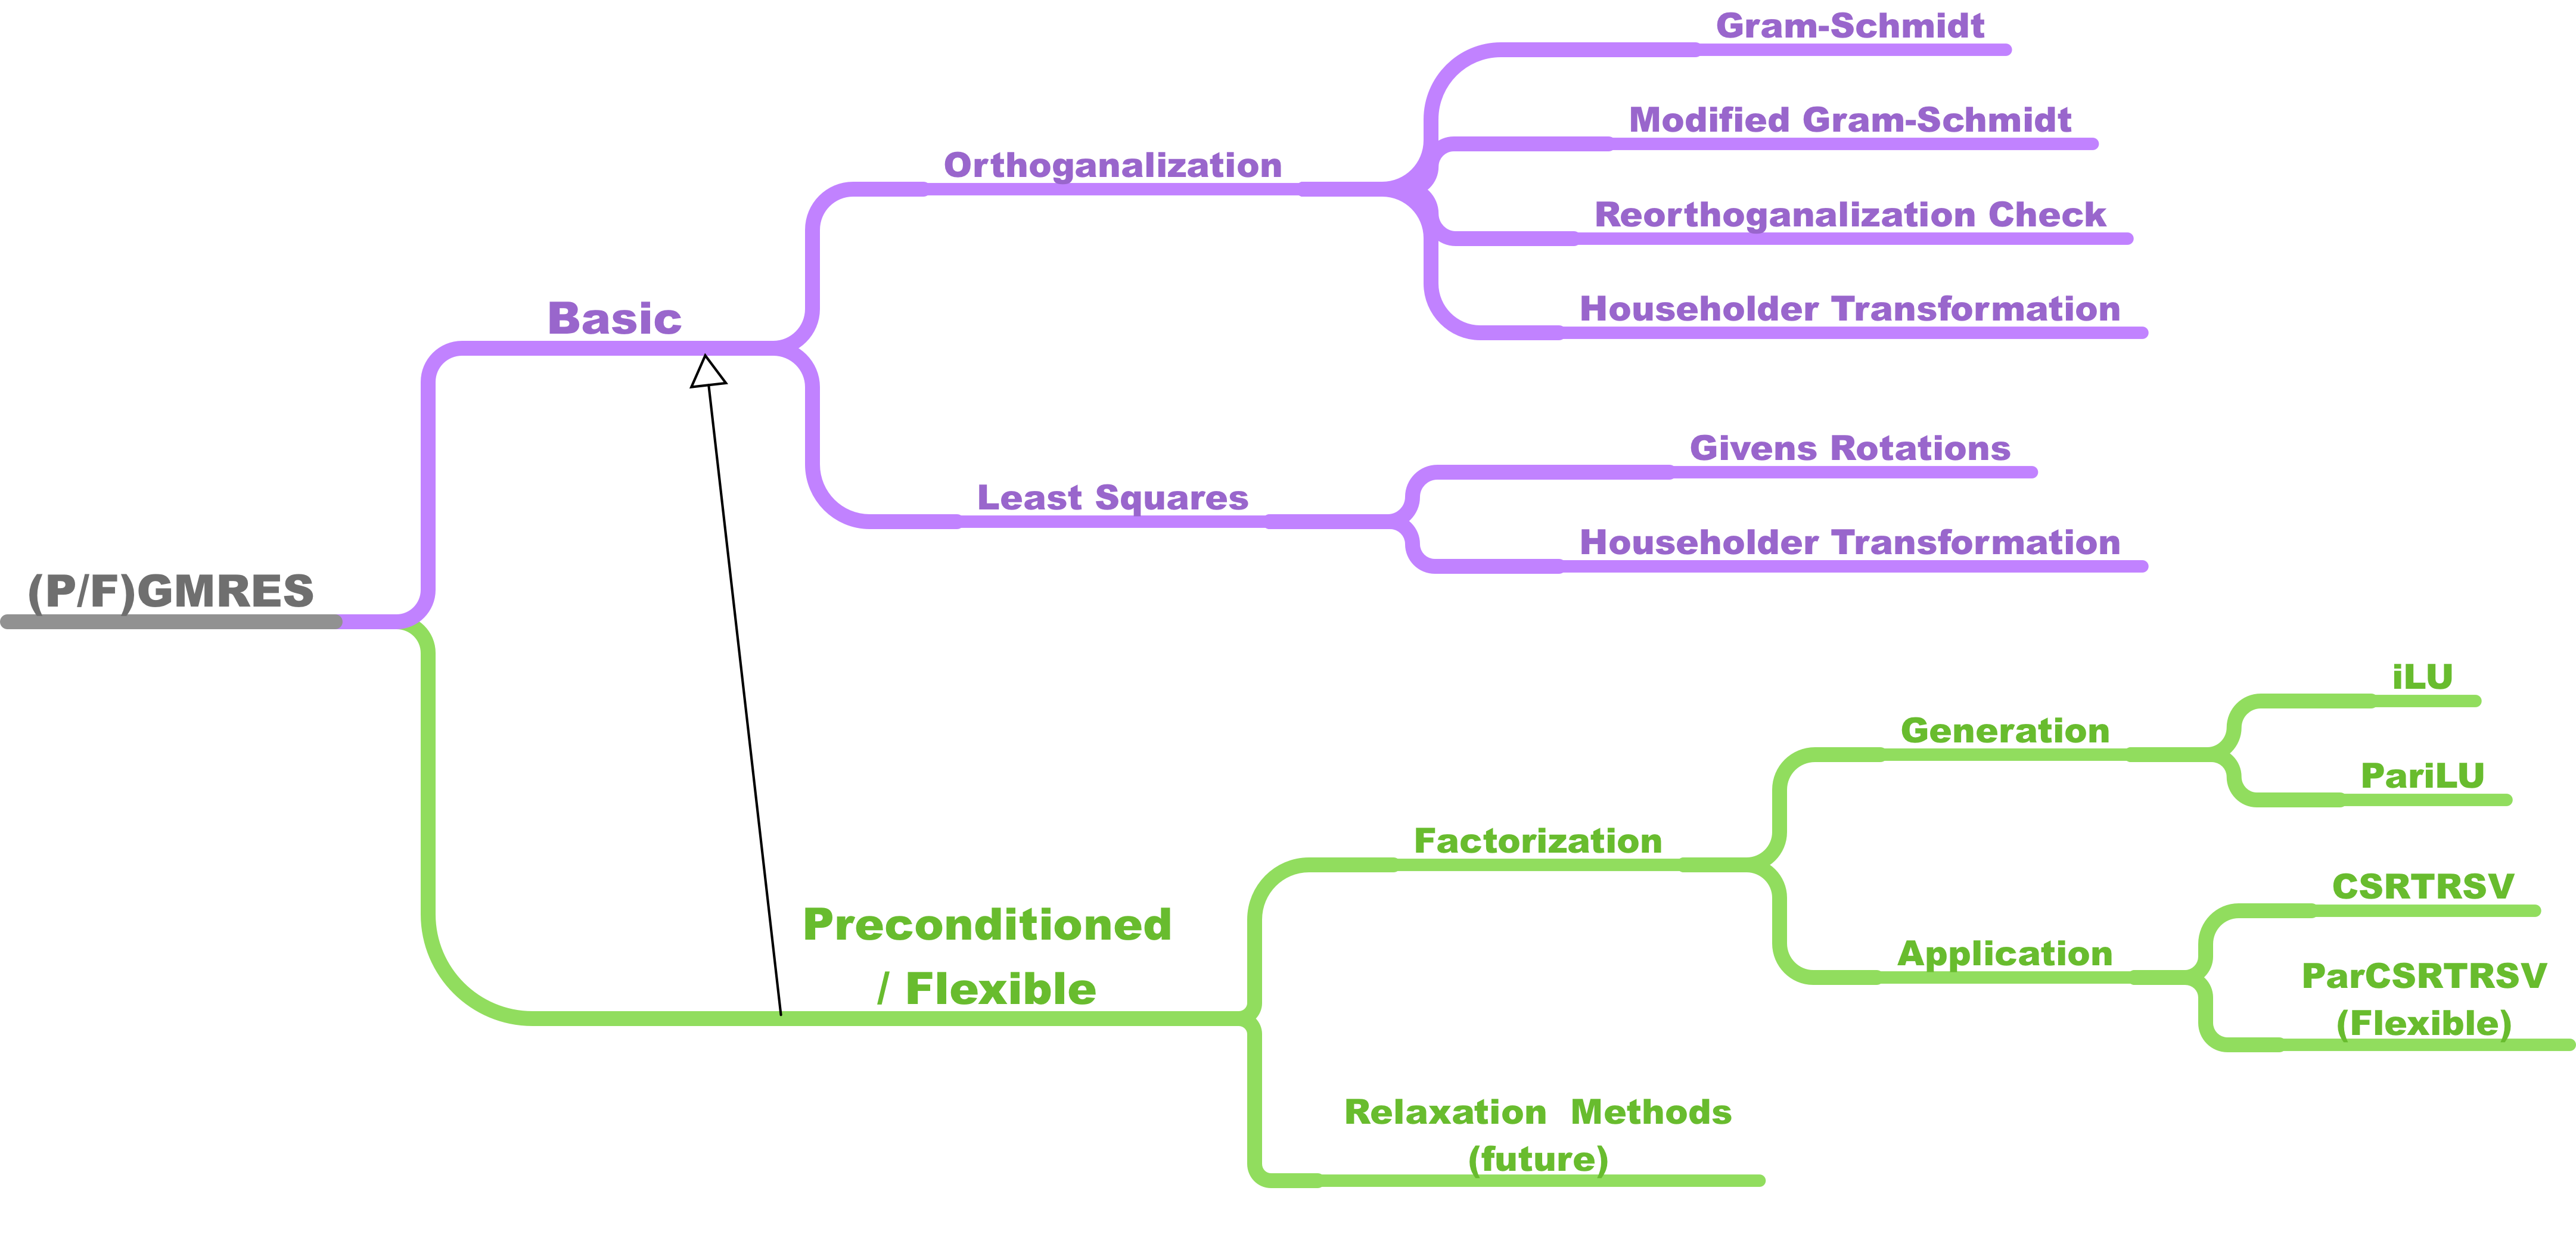
\includegraphics[width=\columnwidth]{../images/GMRES_1b.png}
  \caption{Outline of Generalized Minimal Residual Method implementation within LACE.}
  \vspace{-10pt}
  \label{fig:LACE_GMRES}
\end{sidewaysfigure}

\FloatBarrier
\section{Test Problem}

Variants of the GMRES solver implemented within LACE have been applied to the 30p30n 
multi-component airfoil benchmark problem from the BANC-II 
workshop to examine the impact of preconditioner generation and application in serial and parallel.
The domain discretization is shown in Figure \ref{fig:30p30n_domain}.
The solution and matrix are visualized int Figure \ref{fig:30p30n_solution}.

\begin{figure}[ht]\centering
 \begin{tabular}{cc}
 \multirow{2}{*}{
  \begin{subfigure}[!ht]{0.5\textwidth}
        \centering
  \vspace{-60pt}
  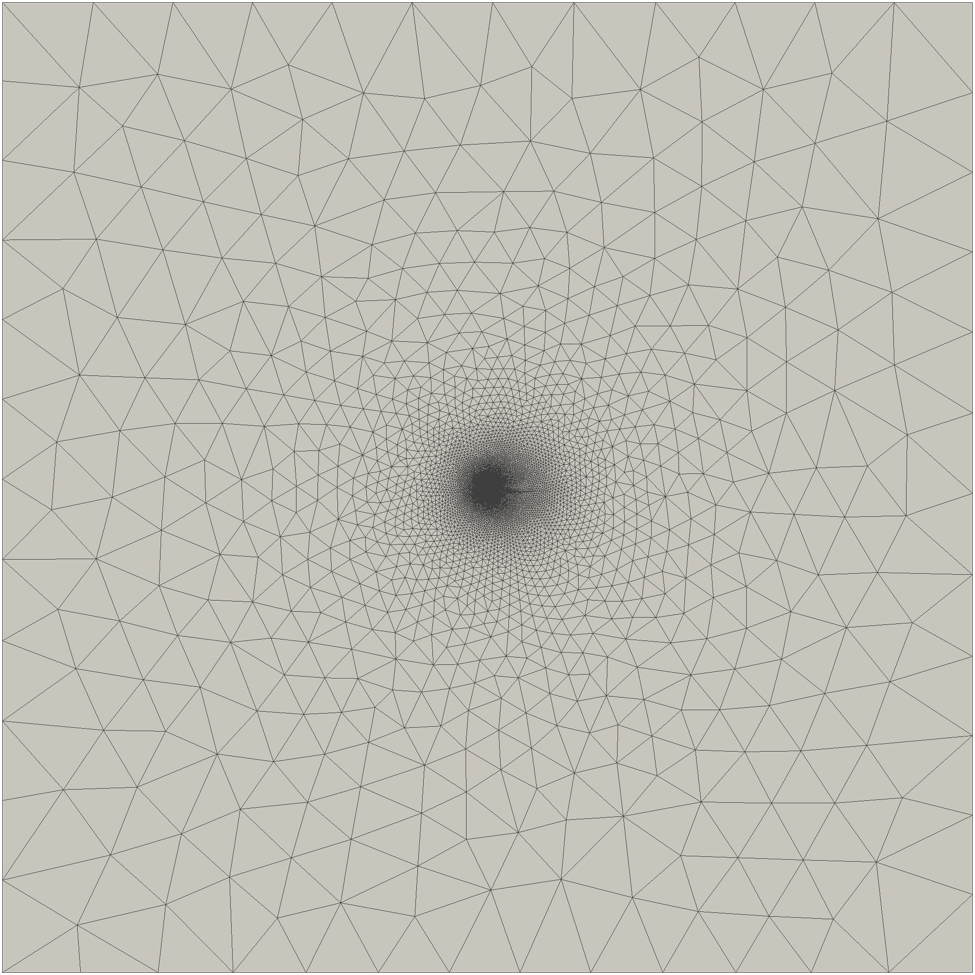
\includegraphics[width=\columnwidth]{../images/30p30n_entireDomain.png}
  \caption{Entire domain.}
  \label{fig:30p30n_convergence}
  \end{subfigure}%
  }
   &
    \begin{subfigure}[!ht]{0.5\textwidth}
        \centering
        \vspace{5pt}
  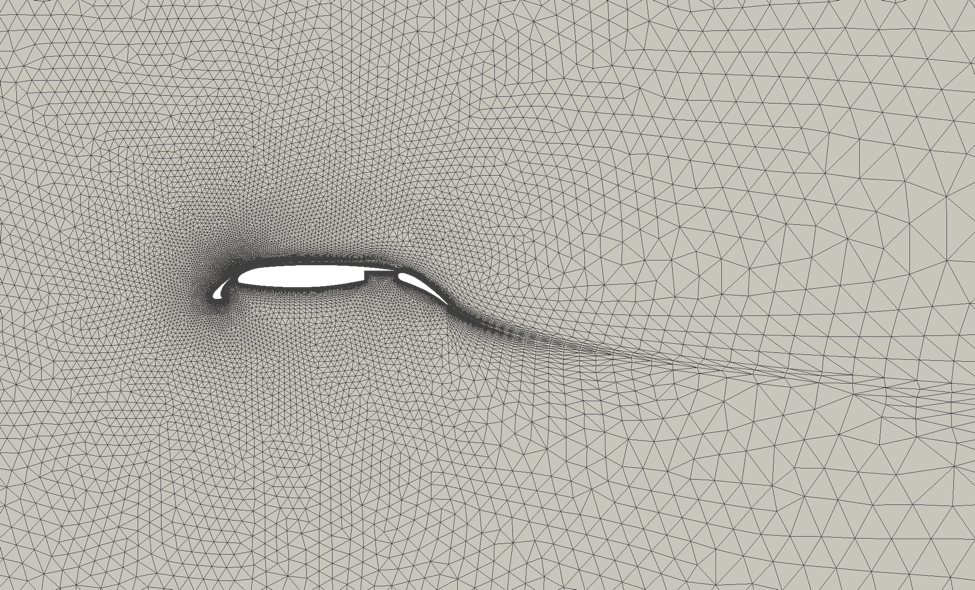
\includegraphics[width=0.99\columnwidth]{../images/30p30n_zoom1.png}
  \caption{Enlarged view of the near ware region.}
  %\vspace{-10pt}
  \label{fig:30p30n_zoom1}
  \end{subfigure}% 
  \\
  &
  \begin{subfigure}[!hb]{0.5\textwidth}
        \centering
  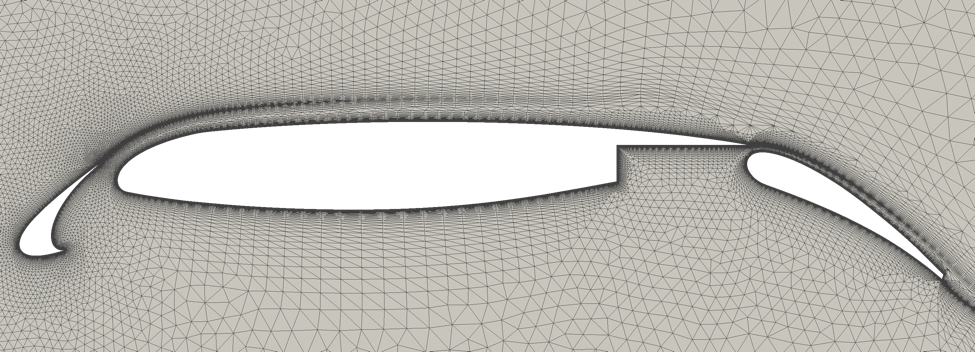
\includegraphics[width=0.99\columnwidth]{../images/30p30n_zoom2.png}
  \caption{Enlarged view of the geometry and boundary layer elements.}
  %\vspace{-10pt}
  \label{fig:30p30n_zoom2}
  \end{subfigure}%
  \\
  \end{tabular}
  \caption{Domain discretization for the 30p30n multi-component airfoil benchmark problem.}
  \label{fig:30p30n_domain}
\end{figure}


\begin{figure}[ht]\centering
   \begin{subfigure}[!ht]{0.5\textwidth}
        \centering
  \vspace{-60pt}
  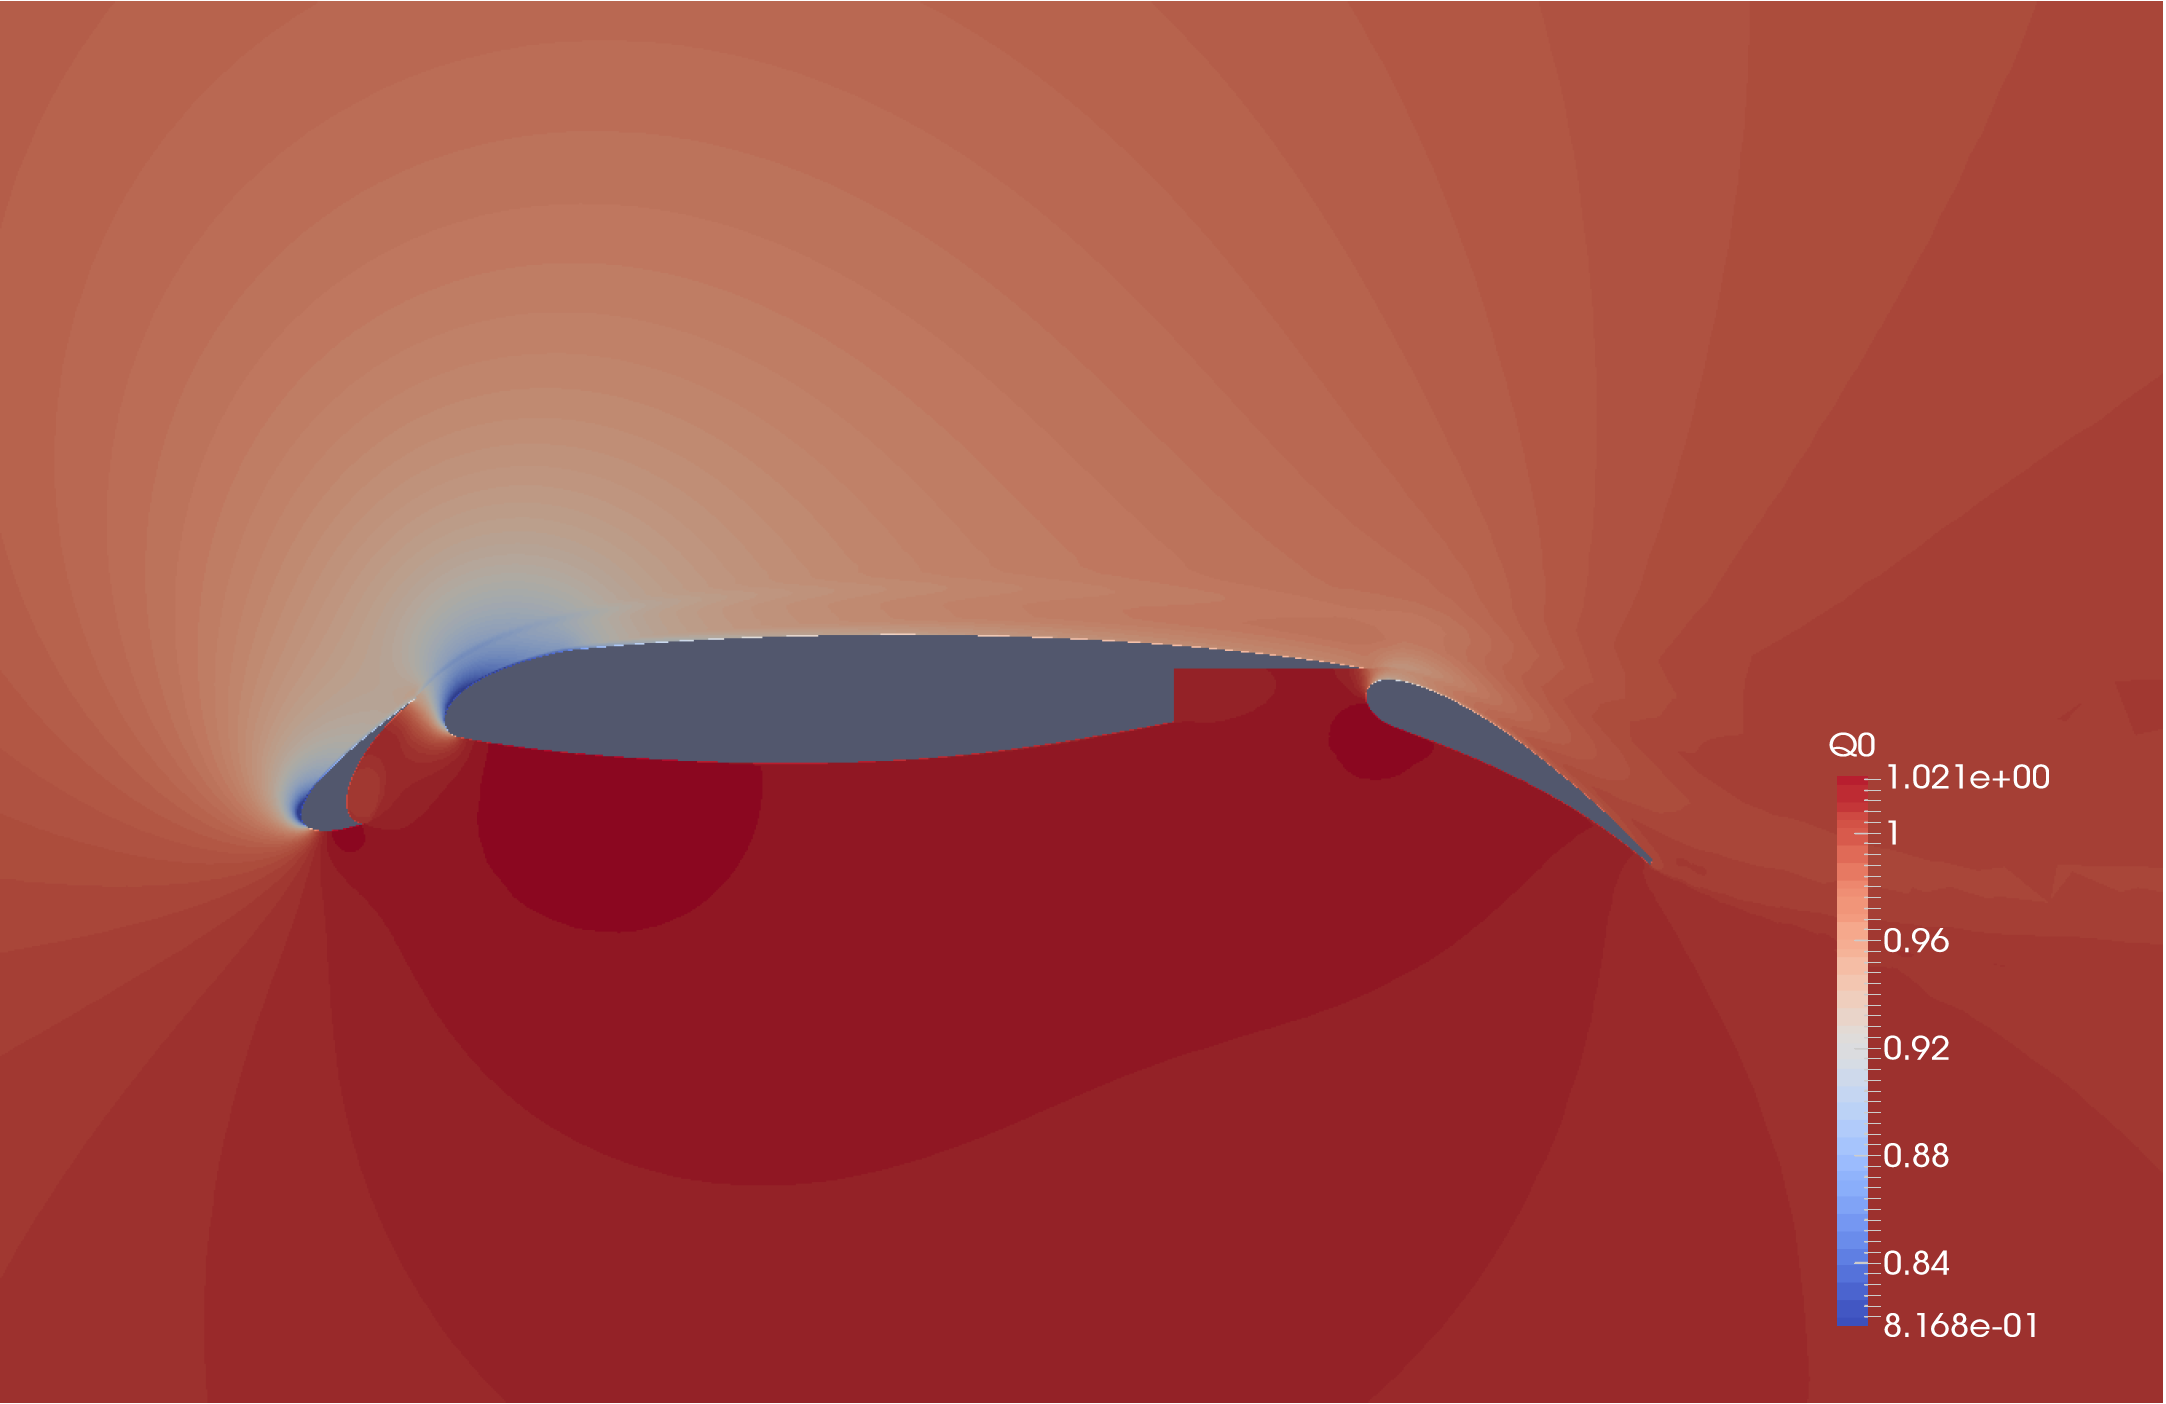
\includegraphics[width=\columnwidth]{../images/30p30n_non-dim_density.png}
  \caption{Visualization of non-dimensionalized density field.}
  \label{fig:30p30n_non-dim_density}
  \end{subfigure}%
  ~
   \begin{subfigure}[!ht]{0.5\textwidth}
        \centering
  \vspace{-60pt}
  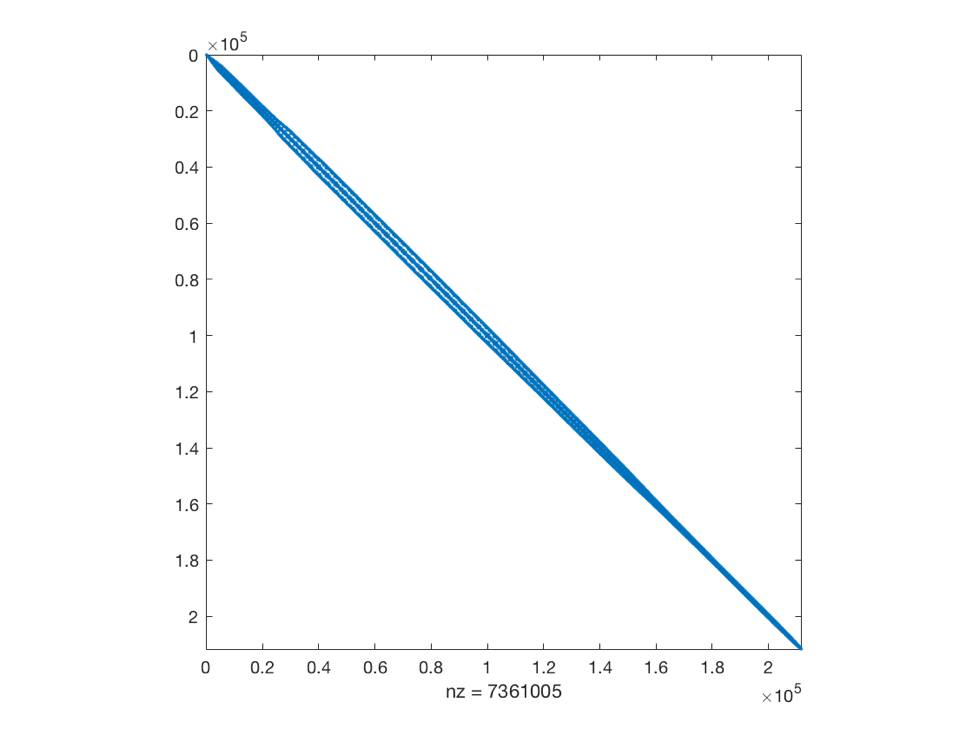
\includegraphics[width=\columnwidth]{../images/30p30n_sparsity.png}
  \caption{Sparsity pattern of coefficient matrix for the simulation.}
  \label{fig:30p30n_sparsity}
  \end{subfigure}%
  \caption{Visualization of the flow around the multi-component airfoil in physical space in juxtaposition with the matrix of coefficients.}
  \label{fig:30p30n_solution}
\end{figure}

The results shown in Figure \ref{fig:30p30n_convergence} were generated with a MacBook Pro (Mid 2014) while the Beacon cluster at the JICS 
Advanced Computing Facility was undergoing maintenance. 
Eight OpenMP threads were utilized for preconditioner generation by the Parallel incomplete LU 
(PariLU) factorization algorithm. 
Eight OpenMP threads were also utilized for preconditioner application by the Parallel Compressed 
Sparse Row Triangular Solves (ParCSRTRSV) algorithms.
\\
It should be noted that orthogonalization was carried out with the Modified Gram-Schmidt algorithm and Givens Rotations were applied to solve the least squares problem within the Flexible GMRES

\begin{figure}[ht]\centering
  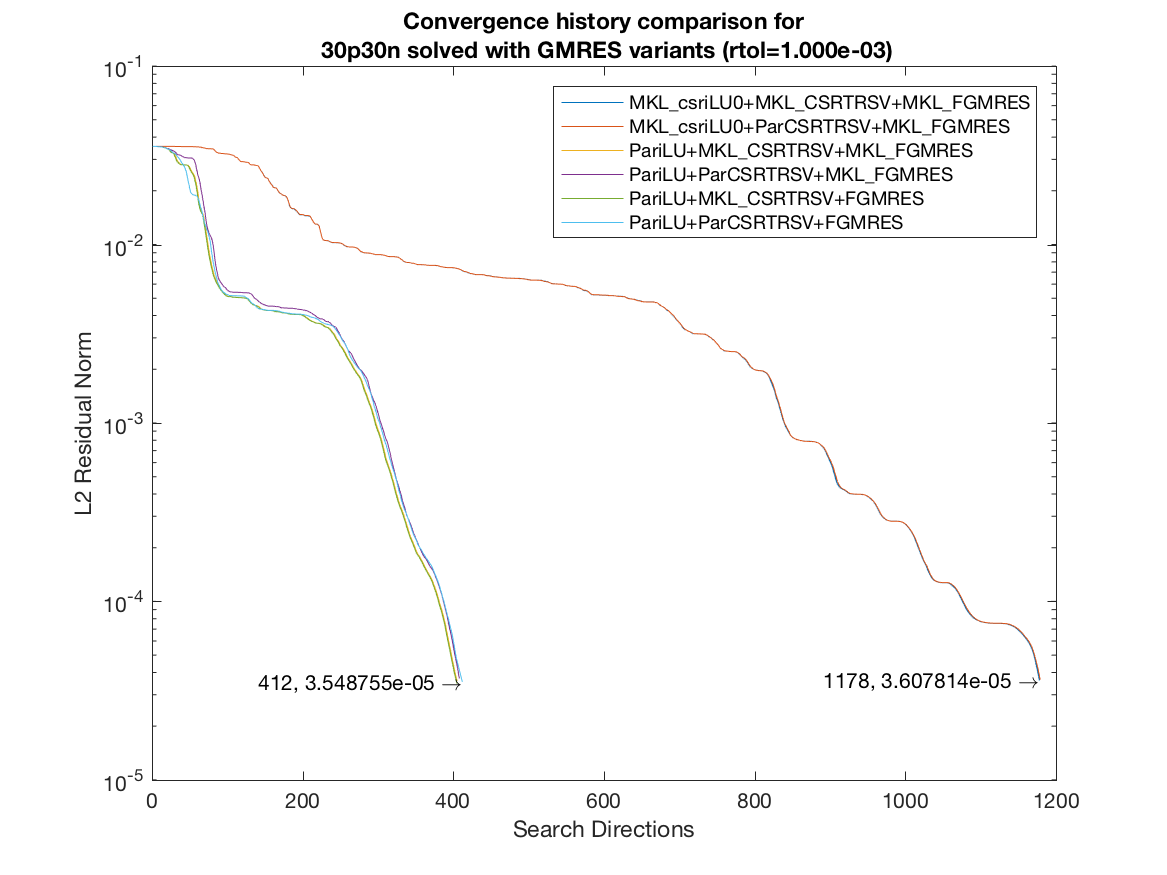
\includegraphics[width=0.95\columnwidth]{../images/30p30n_compare_GMRES_convergence_hist.png}
  \caption{Comparison of convergence history for a sampling of Flexible GMRES variants implemented to date within LACE and the Intel MKL 2017 FGMRES Method.}
  \vspace{-10pt}
  \label{fig:30p30n_convergence}
\end{figure}




\end{document}


